\documentclass[letterpaper]{article}

%pass the page height/width into pdflatex, otherwise it assumes A4
\pdfpagewidth=\paperwidth
\pdfpageheight=\paperheight

\usepackage{graphicx} %get graphics commands
\usepackage{times}

%get \FloatBarrier command
\usepackage{placeins} 

%give option to use commands like 0.5\textwidth for distances
\usepackage{calc} 
 %allows wraping figures around text
\usepackage{wrapfig}

%adds option to include verbatim input from files
\usepackage{moreverb} 

%Set the pages margins to 1 inch, all the way around
\usepackage{anysize}
\marginsize{1in}{1in}{0.45in}{0.45in}

\begin{document}

\begin{figure}[htbp]
\begin{center}
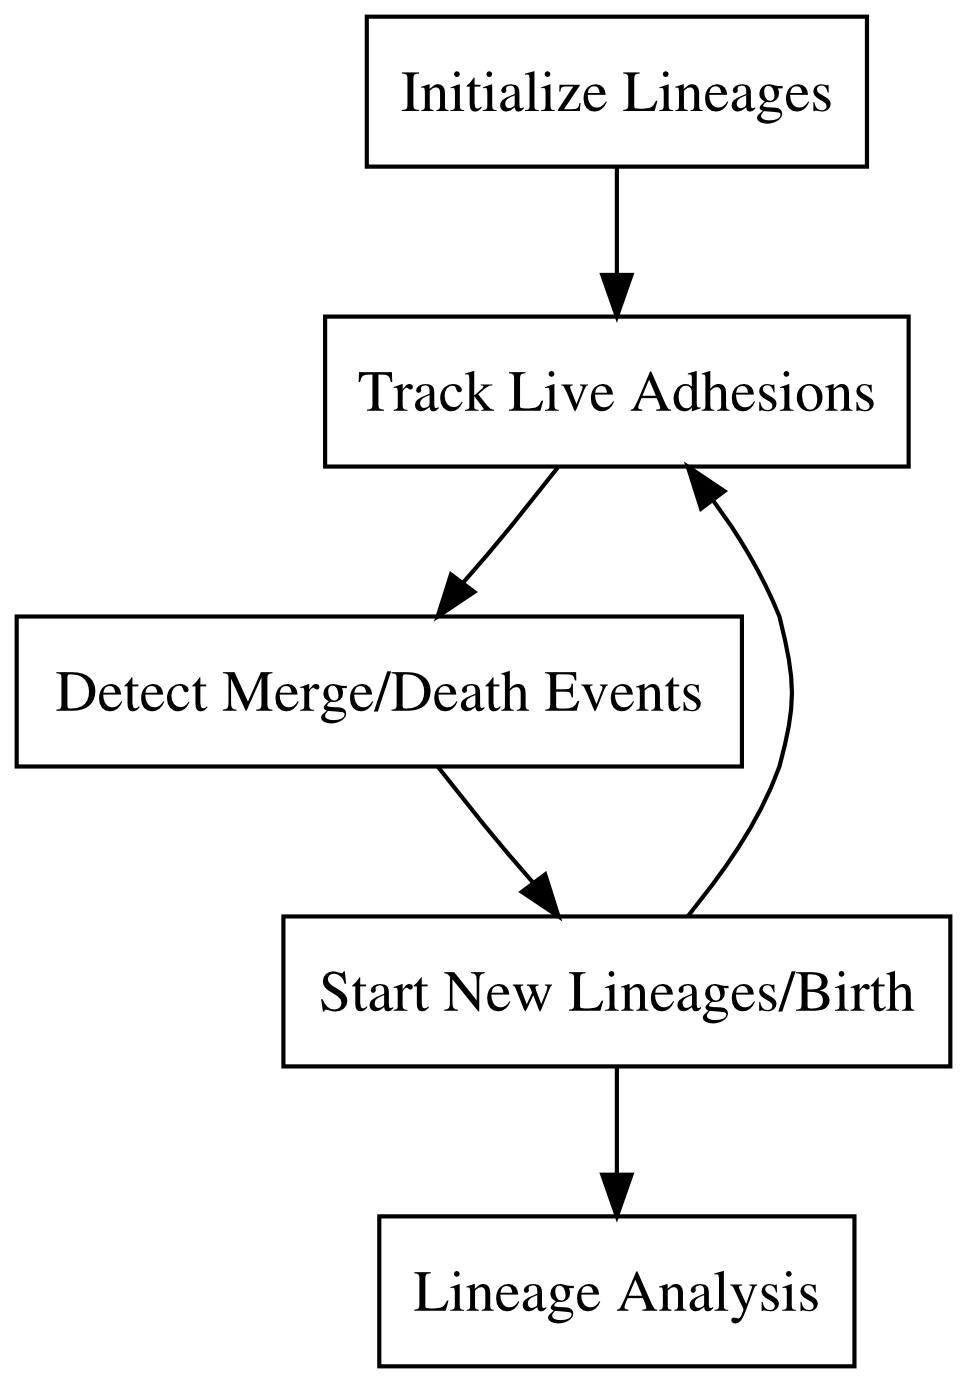
\includegraphics{../figures/supplemental/tracking_flowchart}
\caption{The tracking software is based around a simple model of FA birth and
death. The tracking software is initialized with all the adhesions in the first
frame. In the transition between frames, an FA can continue living, merge with
another adhesion, die or be born. The first set of decisions involves tracking
all the living adhesions, i.e. assigning current adhesions to their most likely
match in the following movie frame. This assignment often causes the adhesions
to be predicted to merge, which is collapsed in software to one of the adhesions
becoming the new merged adhesion. The other adhesions involved in the merge
event are predicted to die, but with their death events marked as a merge. The
death events are also detected in this step. Finally, any adhesion not predicted
to be an adhesion from the current frame is detected and added has having been
born between the two frames.}
\label{default}
\end{center}
\end{figure}

\begin{figure}[htbp]
\begin{center}
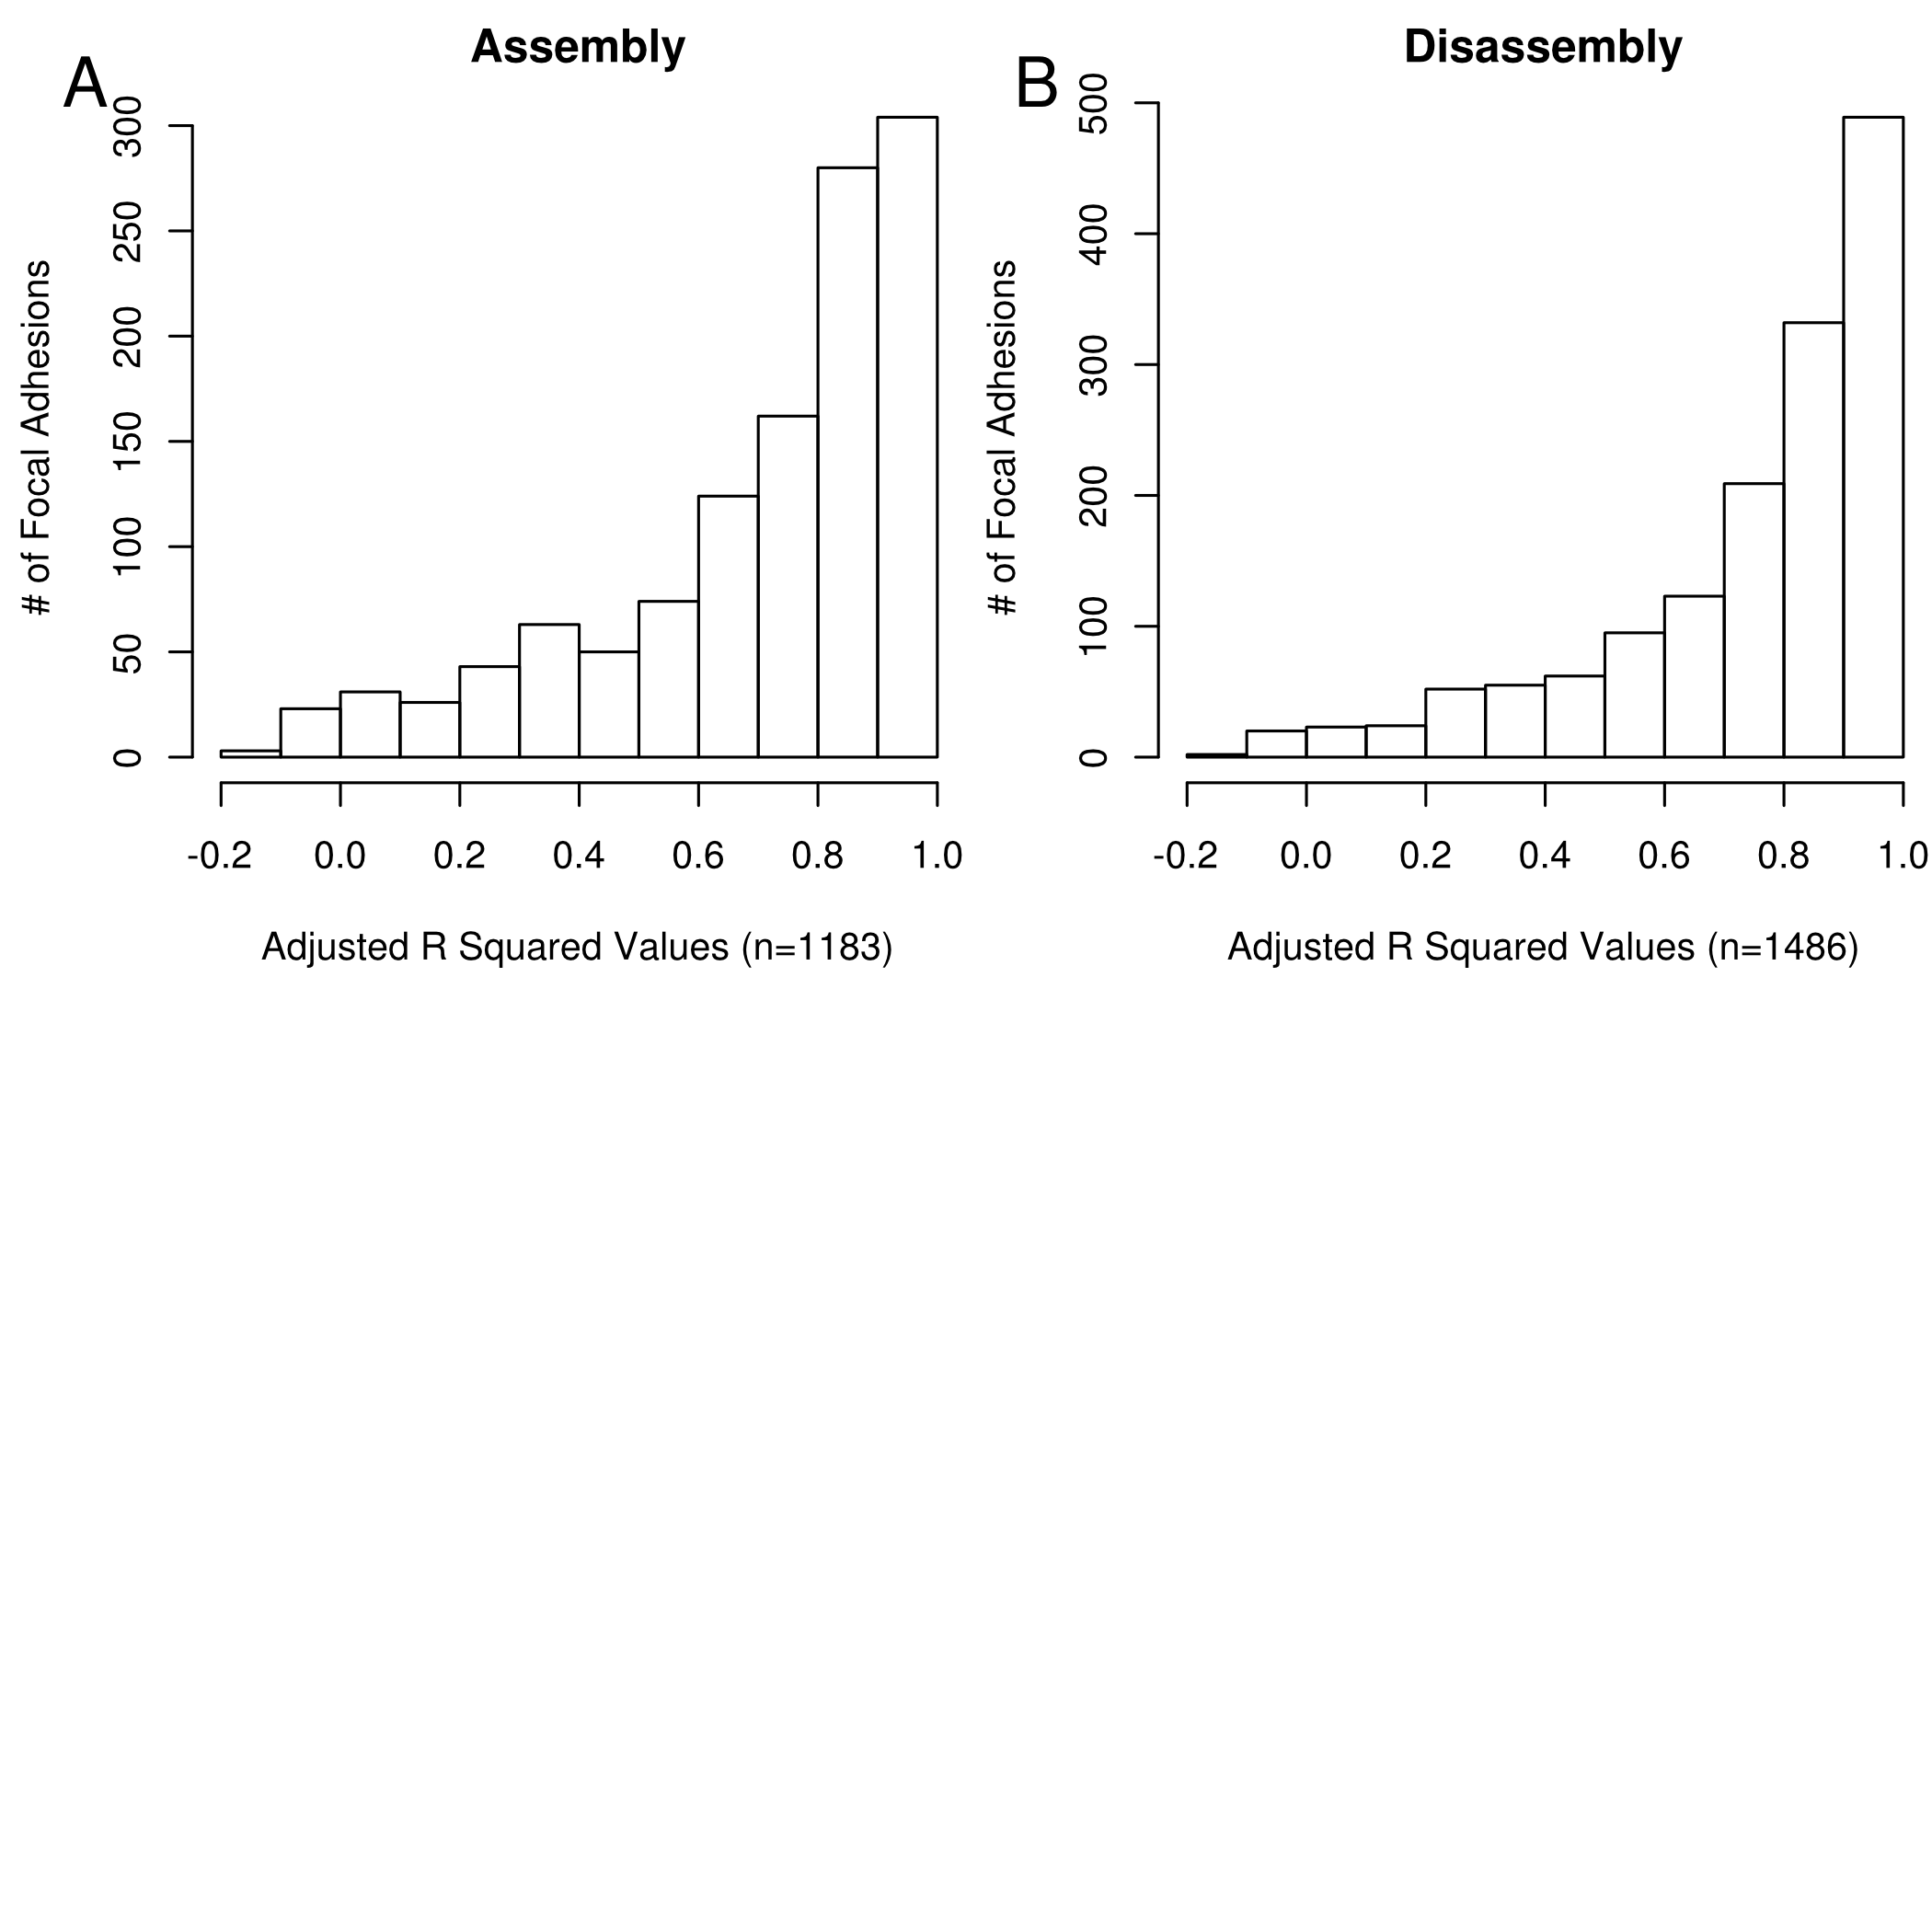
\includegraphics[width=\textwidth]{../figures/supplemental/R_squared}
\caption{The assembly and disassembly log-linear models fit the Paxillin
intensity time courses with high R$^2$ values. Fifty percent of the R$^2$ values
lie above 0.796 in the assembly fits and 0.833 in the disassembly fits.}
\label{default}
\end{center}
\end{figure}

\begin{figure}[htbp]
\begin{center}
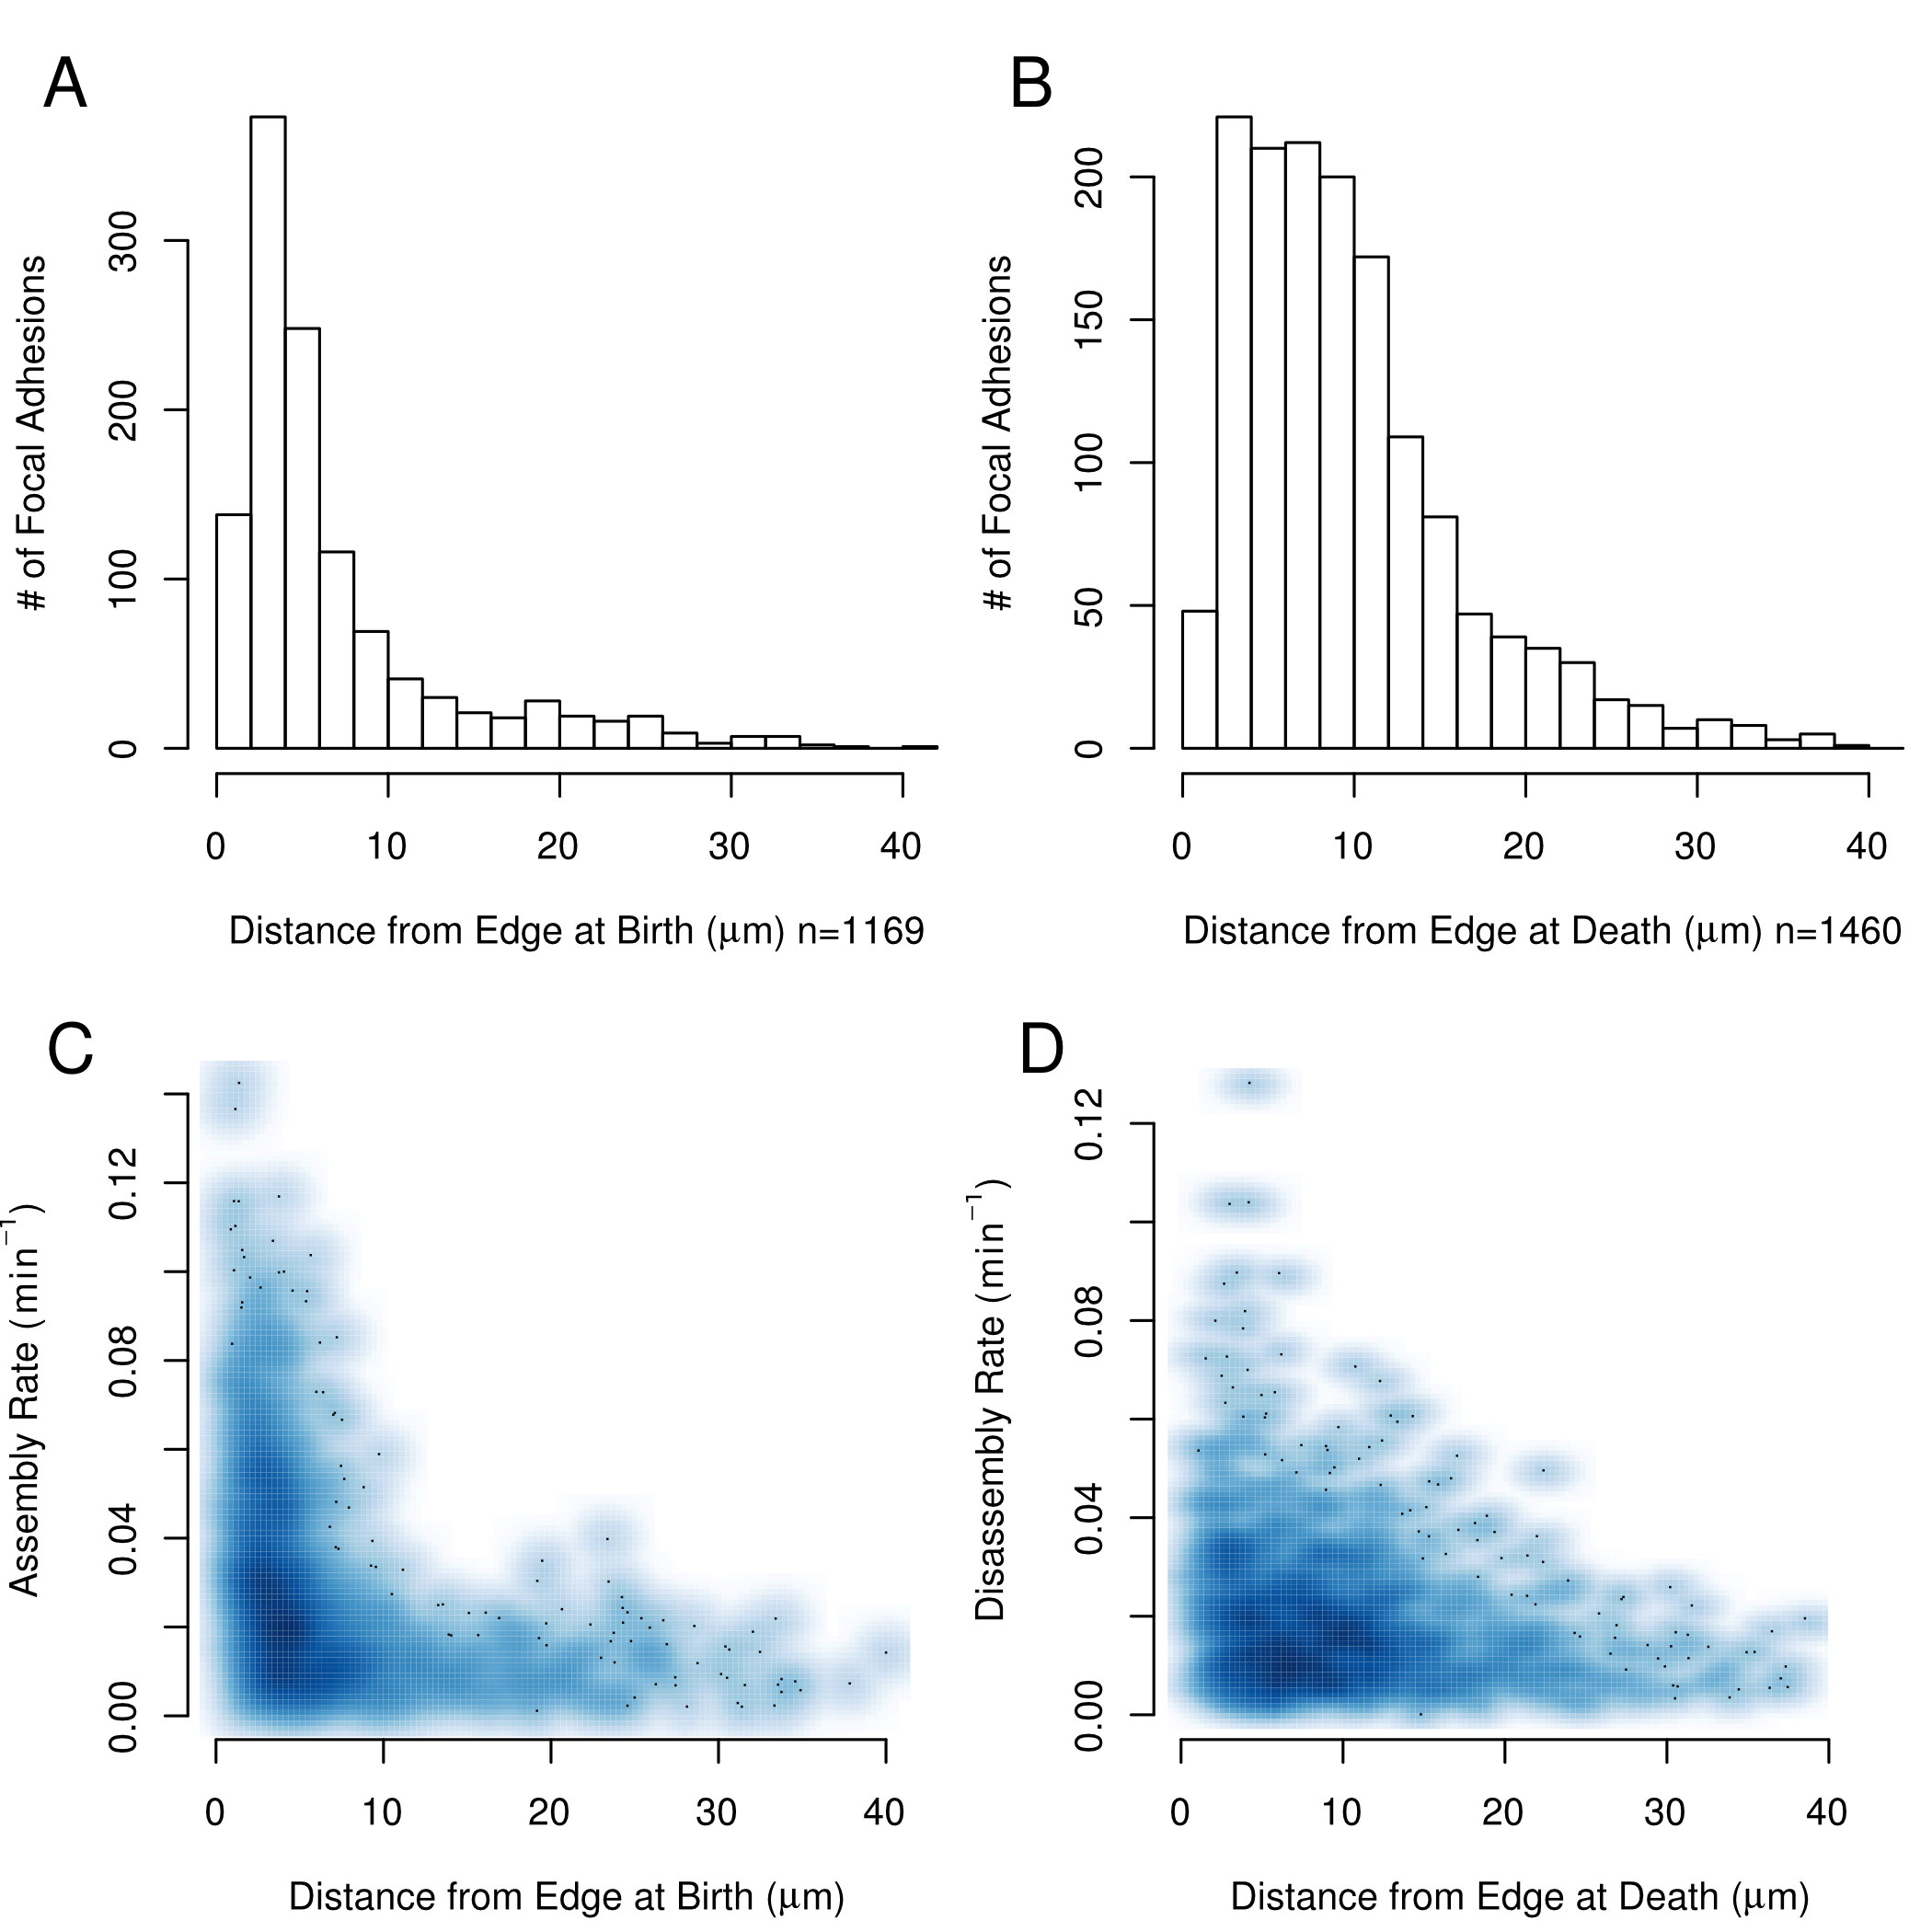
\includegraphics[width=\textwidth]{../figures/supplemental/spacial_nofilt}
\caption{Adhesions assembly and disassembly occurs in two overlapping bands as
identified by the distance from the cell edge. This is the same pattern as
seen in the filtered data set.}
\label{default}
\end{center}
\end{figure}

\begin{figure}[htbp]
\begin{center}
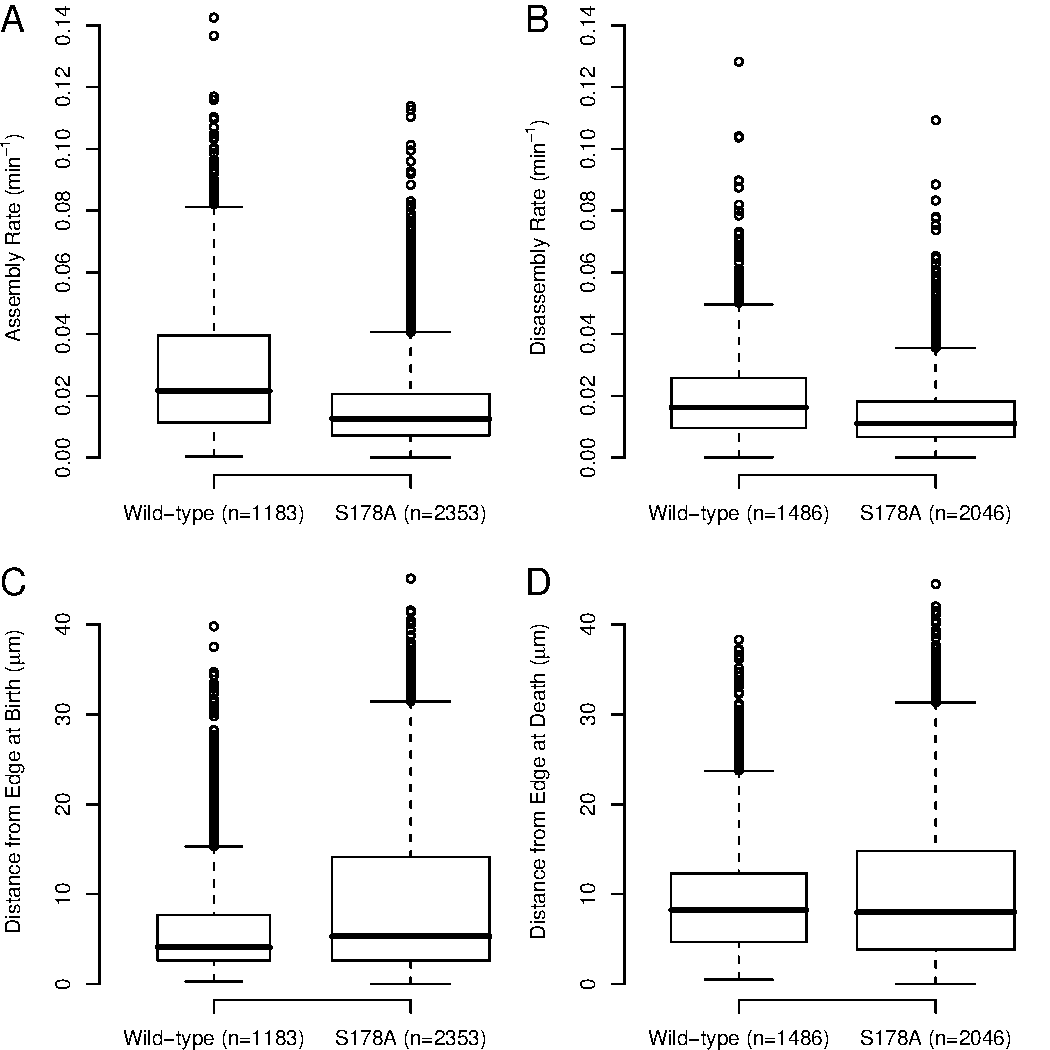
\includegraphics{../figures/supplemental/unfilt_S178A_vs_wild-type}
\caption{The S178A mutant of Paxillin perturbs several measure of FA
development. The data in these boxplots are the data filtered to only include
significant log-linear model fits (p-value less than 0.05). The same patterns
hold in comparing the unfiltered to the filtered wild-type and S178A data sets.}
\label{default}
\end{center}
\end{figure}

\end{document}
